\section{Introduction}


The \textit{pooling} operation is central to the convolutional neural network (CNN). It was originally introduced in the first CNN architecture\textemdash Fukushima's 1980 \textit{Neocognitron}~\cite{fukushima1980}\textemdash and remained a fixture of the model since. The Neocognitron was directly inspired by the canonical model of the visual cortex as a process of hierarchical feature extraction and local pooling~\cite{hubel1959receptive, adelson1985spatiotemporal}. In both the neuroscience and CNN model, pooling is intended to serve two purposes. First, it facilitates the local-to-global \textit{coarse-graining} of structure in the input. Second, it facilitates \textit{invariance} to local changes\textemdash resulting in network activations that remain similar under small perturbations of the input. In this way, CNNs construct hierarchical, multi-scale features that have increasingly large extent and increasing invariance.

The pooling operation in traditional CNNs, typically a local max or average, has remained largely unchanged over the last forty years. The variations that have been proposed in the literature~\cite{Nirthika2022,Zafar2022} mostly tackle its \textit{coarse-graining} purpose, improve computational efficiency, or reduce overfitting, but do not seek to enhance its properties with respect to \textit{invariance}. Both \texttt{max} and \texttt{avg} operations are reasonable choices to fulfill the goal of coarse-graining within CNNs and $G$-CNNs. However, they are excessively imprecise and lossy with respect to the goal of constructing robust representations of objects that are invariant only to irrelevant visual changes. Indeed, the \texttt{max} and \texttt{avg} operations are invariant to many natural image transformations such as translations and rotations, but also to unnatural transformations, including pixel permutations, that may destroy the image structure. This excessive invariance has been implicated in failure modes such as vulnerability to adversarial perturbations~\cite{goodfellow2014explaining,jacobsen2018excessive}, and a bias towards textures rather than objects~\cite{brendel2019approximating}. To overcome these challenges and enable robust and selective invariant representation learning, there is a need for novel computational primitives that selectively parameterize invariant maps for natural transformations.

% Beyond traditional CNNs, the more recent group convolutional neural networks ($G$-CNNs) seek to achieve equivariance with respect to a group of transformations that extend the group of translations. In this line of work, invariance to the group $G$ is standardly achieved by generalizing the concept of max pooling, with Max $G$-Pooling~\cite{cohen2016group}.

% At the heart of the challenge lie two requirements that are frequently in tension: \textit{invariance} to transformation structure and \textit{selectivity} to pattern structure. In deep networks, operations such as \texttt{max} or \texttt{average} are commonly employed to achieve invariance to local transformations. Such operations are invariant to many natural transformations; however, they are also invariant to unnatural transformations that destroy image structure, such as pixel permutations. This lack of selectivity may contribute to failure modes such as susceptibility to adversarial perturbations \cite{goodfellow2014explaining}, excessive invariance \cite{jacobsen2018excessive}, and selectivity for textures rather than objects \cite{brendel2019approximating}. Thus, there is a need for computational primitives that selectively parameterize natural transformations and facilitate robust invariant representation learning.

Many of the transformations that occur in visual scenes are due to the actions of \textit{groups}. The appreciation of this fact has led to the rise of group-equivariant convolutional networks ($G$-CNNs) \cite{cohen2016group} and the larger program of Geometric Deep Learning \cite{bronstein2021geometric}. While this field has leveraged the mathematics of group theory to attain precise generalized group-equivariance in convolutional network layers, the pooling operation has yet to meet its group theoretic grounding. Standardly, invariance to a group $G$ is achieved with a simple generalization of max pooling: Max $G$-Pooling~\cite{cohen2016group} \textemdash see Fig.~\ref{fig:overview-cnn-c4} (top-right). However, this approach inevitably suffers from the lossiness of the \texttt{max} operation.

Here, we unburden the pooling operation of the dual duty of invariance and coarse-graining, by uncoupling these operations into two steps that can be performed with precision. We retain the standard \texttt{max} and \texttt{avg} pooling for coarse-graining, but introduce a new method for robust $G$-invariance via the group-invariant triple correlation \textemdash see Fig.~\ref{fig:overview-cnn-c4} (bottom-right). The group-invariant triple correlation is the lowest-order complete operator that can achieve exact invariance~\cite{kakarala1992triple}. As such, we propose a general framework for robust $G$-Invariance in $G$-Equivariant Networks.
%the spatial dual of the bispectrum \cite{kakarala2012bispectrum}.
%^^Removed to avoid scaring people (from bioshape comments).
We show the advantage of this approach over standard max $G$-pooling in several $G$-CNN architectures. Our extensive experiments demonstrate improved scores in classification accuracy in traditional benchmark datasets as well as improved adversarial robustness.

\begin{figure}
    \centering
    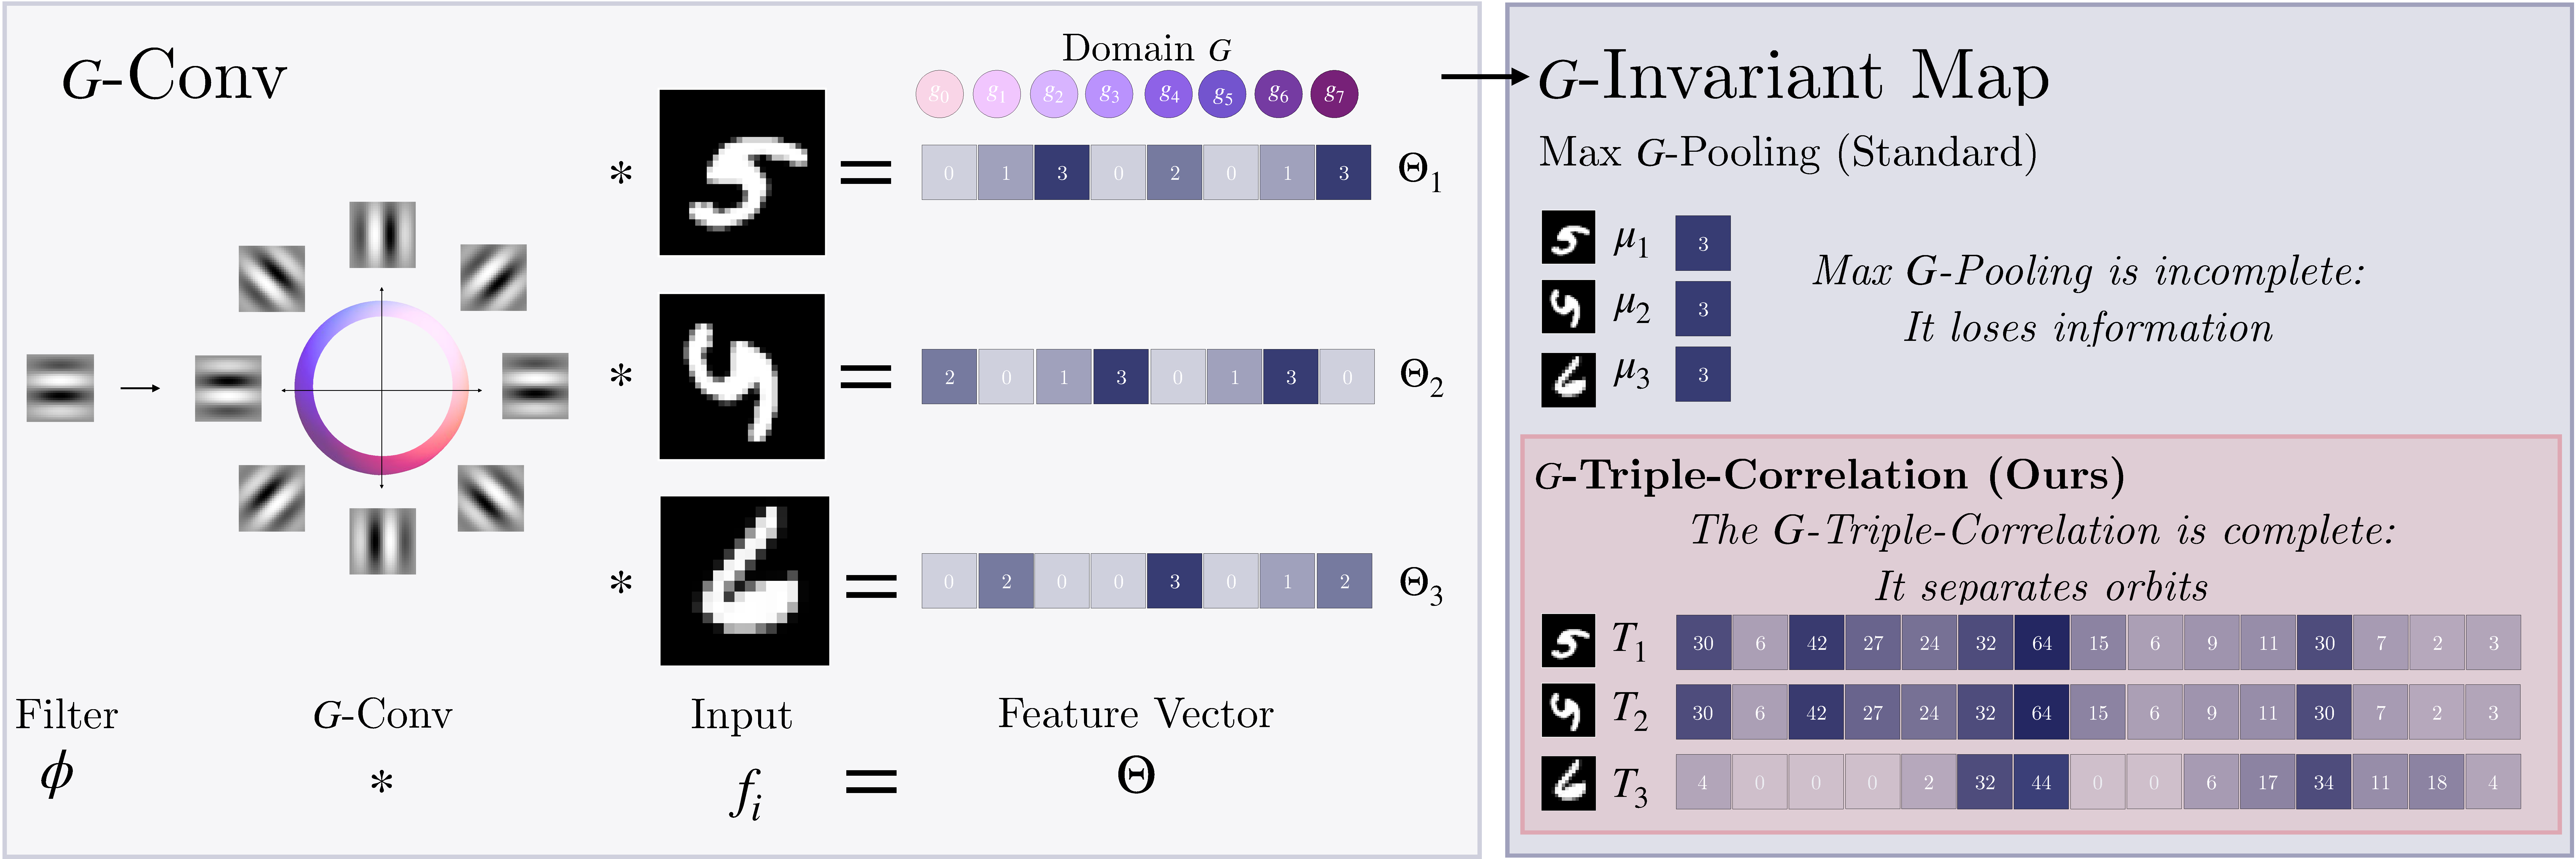
\includegraphics[width=1\textwidth]{figs/master-figure-complex-2.pdf}
    \caption{\textbf{Achieving Robust $G$-Invariance in $G$-CNNs with the $G$-Triple-Correlation}. The output of a $G$-Convolutional layer is equivariant to the actions of $G$ on the domain of the signal.  To identify signals that are equivalent up to group action, the layer can be followed by a $G$-Invariant map that eliminates this equivariance. In $G$-CNNs, Max $G$-Pooling is a commonly used for this purpose. Taking the maximum of the $G$-Convolutional equivariant output is indeed invariant to the actions of the group. However, it is also lossy: many non-equivalent output vectors have the same maximum. Our method\textemdash the \textit{$G$-Triple-Correlation} is the lowest-order polynomial invariant map that is \textit{complete} \cite{sturmfels2008algorithms}. As a complete invariant, it preserves all information about the signal structure, removing only the action of the group. Our approach thus provides a new foundation for achieving robust $G$-Invariance in $G$-CNNs.}
    \label{fig:overview-cnn-c4}
\end{figure}


% Indeed, they are \textit{invariant} to transformations; however, they are \textit{too} invariant.

% : the down-sampling of representations in the network, by collapsing local regions.
